\documentclass[./dissertation.tex]{subfiles}
\begin{document}


 
%%%%%%%%%%%%%%%%%%%%%%%  TIMER  %%%%%%%%%%%%%%%%%%%%%%%%%%%


  \section{Timer}

\label{timer_sec}
In this section, a timer IP block will be designed. The functionalities of the timer are inspired by the ST's timers \cite{TimerManualSTM}. The functionalities should cover a large number of general use cases. The timer will consist of two functional parts: the counter and multiple capture/compare registers. To describe the functionalities which need to be implemented in these two functional units, a list has been made which can be seen below.

\begin{itemize}
    \item 16-bit up/down, on-the-fly adjustable auto reload counter capable of counting center-aligned modes (CMS).
    \item 16-bit prescaler on-the-fly adjustable.
    \item 4 independent capture/compare channels with on-the-fly update.
    \item Capture, compare equality, compare greater than, compare toggle \& one-pulse mode for the capture/compare registers (CCR)
    \item Interrupt generation on update event, trigger event, input capture or output compare.
    \item Input capture filter and edge detector.
\end{itemize}

These features will now be elaborated to ensure a common understanding:

\begin{itemize}
    \item Update event (UEV): Describes when the main counter inside the timer is reset, either from overflow or underflow.
    \item Auto-reload: Gives the attached counter the ability to reset to or on the value of this register, depending on the counter mode.
    \item On-the-fly adjustable: Normally the auto-reload value, the prescaler value, and the CCR value would be synchronized to update on a UEV, however using on-the-fly it is possible to update these values in the middle of counting progress.
    \item Center-aligned modes: refers to a operational mode of counter where it automatically switches between counting up and down every time it overflows/underflows. There are 4 different modes depending on which direction it should update the output. 
    \item (Input) Capture: refers to an external event triggering a capture thereby saving the value of the counter into the CCR.
    \item (Output) Compare: refers to the comparison between the CCR value and the counter value, when a specified criterion is met, i.e the counter value is greater than or equal to the CCR value, then a specified output signal is asserted.
    \item One-pulse Mode: refers to the system creating a single pulse at a specified time and then ending it at another specified time and stopping either the counter itself or disabling the relevant CCR.
\end{itemize}

From this list of features, a figure is constructed showing the different high-level blocks of the timer, which is seen in \ref{fig:timer_block_dia}. 

\begin{figure}[H]
    \centering
    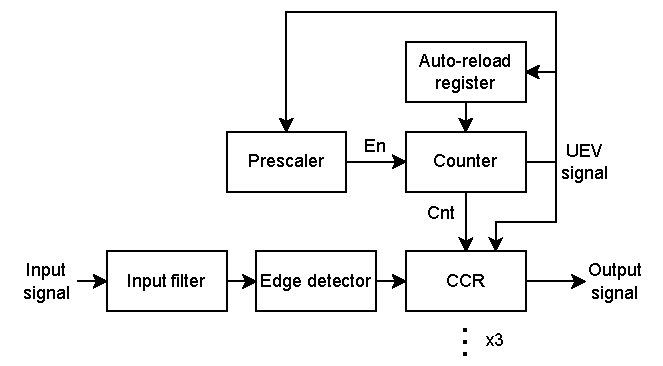
\includegraphics[width = 0.8\linewidth]{subfiles/imgs/IP_Blocks_Pics/timer_block_dia.drawio.pdf}
    \caption{Shows the functional blocks of the timer. The CCR register is repeated 3 times, for a total of 4 CCR registers.}
    \label{fig:timer_block_dia}
\end{figure}

A list of control registers is used to program the timer to the intended application. A detailed description of all programmable registers and status register can be found in the RDL file for the timer in the GitHub repository.

The amount of capture/compare registers is potentially unlimited, however it is chosen to use 4 as a standard following the ST Microelectronics timer \cite{TimerManualSTM}. The development of the timer will be split into two: the timer part consisting of a counter and prescaler, and the capture/compare part.

\subsection{Counter and Prescaler}
The timer itself will have a 16 bit counter as its central component. This counter is a bidirectional, meaning it is capable of both counting up and counting down, which is controlled by a direction signal. Connected to this counter is 16 bit prescaler and a 16 bit auto-reload register. The prescaler is also a 16-bit counter, where the value of reset can be programmed from the APB interface. When the programmed value is reached the prescaler pulls a enable signal high for one clock cycle. The enable signal is sent to the counter, which then counts up/down on the next positive clock edge. Using the prescaler as an enable signal instead of using it to lower the frequency of the system clock, means that no extra clock domains are created, making timing closure easier in the physical implementation. To program the reset value of prescaler, a shadow register is used to ensure that the updating of this value happens at the correct timing. A shadow register is an extra register inserted between the programmable register and the compare circuit used for comparing current count and reset value. Without this, the value would change instantly, the moment the programmable register was written. In some cases this might be preferable, but in other cases control of when this reset value is updated might be needed. This control is implemented in two ways: on-the-fly update and using UEVs as triggers. On-the-fly refers to operation similar to that of using no shadow register resulting in the value being updated instantly, while using UEVs the update will happen when the main counter either overflows and/or underflows.

Besides a prescaler, a 16-bit auto-reload register is also connected to the counter. This auto-reload register controls what value the counter will reset at or reset to depending on the direction. When the counter is counting up it will reset at the value specified in the auto-reload register and when it is counting down it will reset at 0 and take the value of the auto-reload register. This auto-reload register also has a shadow register to control the timing of updating the value. It has the same possible operations as the prescaler, either on-the-fly or on UEVs. Doing CMS mode, the operation of the auto-reload register is different to ensure smooth transistions between counting up and down. For example when the counter is counting up, it will reset at the auto-reload value subtracted one. It then resets to the auto-reload value and inverts the direction bit. When it is counting down, it will reset to 0 and invert the direction bit when the counter has the value 1. This ensures that no value will be repeated in a cycle. 

\subsection{Capture/Compare Register}
The CCR register is the functional unit that generates the output signals of the timer and also receives external signals. The CCR register can be configured to one of these two modes: capture or compare. These modes can be further subdivided or customized to fit the specific application. We will start by discussing the compare part.

The compare part of the CCR generates a output on a single line. This line will continuously switch between logic high and low depending on the operational mode of the CCR, the value to compare against, and the current value of the counter. These things enable the CCR to create a controllable output signal and even enables it to create PWM signals, which are commonly used in control of motors. The value switch the CCR uses to compare against the current counter value is stored in a programmable register equipped with a shadow register identical to that of the prescaler or auto-reload register, such that this compare value can be updated on-the-fly or during an UEV. The operational modes can be controlled by a programmable register and are as follows: deactivated, equal to, greater than, toggle, and one-pulse mode. In "equal to" the output goes high if the compare value is equal to the counter value. In "Greater than" the output goes high if the counter value is greater than the compare value. In "toggle" the output gets inverted every time the compare value is equal to the counter value. In "one pulse mode" the output goes high when the compare value is equal to the counter value and goes low on a UEV. This also deactivates the CCR or the entire counter based on the value in the corresponding programmable register. One has to be aware of the fact that these comparison is not guaranteed to be at all times when the counter is in CMS mode. In this mode the comparison is either done only when counting up or when counting down or at all times. The increase the control of the output a controlled inverter is also added on the output, such that output signal can be programmed to be inverted or not. 

In capture mode, an output is not generated. Instead the CCR waits for a edge on a input line and when this edge is received it saves the current value of the counter into the shadow register of the compare register (The same as used in compare mode). This can be used to generate an interrupt and the value be read through the APB interface. This can be used for a number of things, but most intuitively this can be used to measure the time between two events. To further control the capture mode, a programmable edge detector and a programmable input filter is added. The edge detector goes high when a rising edge or falling edge is detected. This is done by sampling the state of the input signal every clock cycle into a register and comparing this to the current input signal using an AND-gate. If one wish to detect a rising edge, the input of the AND-gate coming from the register should be inverted, while the direct input should not. This way, the AND-gate will go high if the last state of the input signal is low and the current input signal is high. This circuit can be seen in figure \ref{fig:peDetector}. A similar circuit can be made for a falling edge detector. 

\begin{figure}[H]
    \centering
    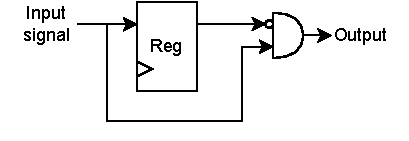
\includegraphics[width = 0.6\linewidth]{subfiles/imgs/IP_Blocks_Pics/edgedetector.drawio.pdf}
    \caption{Shows a positive edge detector circuit. The output will go high when the previous state was 0 and current state is 1, thereby detecting a positive edge.}
    \label{fig:peDetector}
\end{figure}

The input filter is made using a programmable 16-bit counter. This counter will count up if the current input value is equal to the last input value. If they are different it will reset to 0. If it reaches the value in the programmable register of counter it will output the value of the last state. This creates a programmable low-pass filter, which filters out the high frequency digital input signals. If the filter is not enabled, it will simply always pass the current state value.

Before the input signal reaches the input filter, it will have to go through a synchronizer. A synchronizer is needed as the input signal will come from an external source which might be asynchronous to the system clock and can have another clock frequency or clock phase. This is called clock domain crossing (CDC) \cite{cdc_book}. Without a synchronizer this would mean that the input signal could be sampled at a time where setup or hold is violated and a metastable state is induced in the register. This metastable state could then propagate through the CCR and create a fatal error or malfunction. To avoid this a 2 flip-flop synchronizer is used. The is that this gives the input flip-flop time to exit the metastable state and the next flip-flop would then sample a stable flip-flop and thereby avoiding the propagation of the metastable state. However, if the clock frequency is high, the next flip-flop might still sample the first flip-flop in a metastable state. More flip-flops can be added to create a longer synchronizer and decrease the probability of a metastable state propagating. A 2 flip-flop synchronizer will be used here. The resulting circuit of combining the synchronizer and the input filter can be seen in figure \ref{fig:2ff_sync_and_if}. From this figure it is clear that this input filter and synchronizer adds a 4 cycle latency period. However, this delay is known and can therefore be subtracted if necessary. 

\begin{figure}[H]
    \centering
    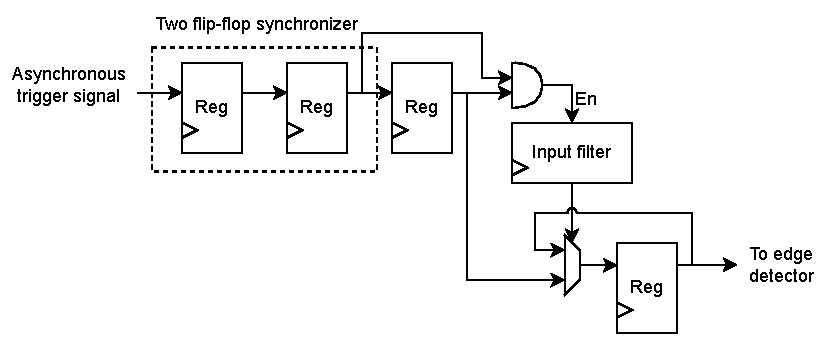
\includegraphics[width = 1\linewidth]{subfiles/imgs/IP_Blocks_Pics/2ffsync.drawio.pdf}
    \caption{Shows the input capture stage with a 2 flip-flop synchronizer and a input filter.}
    \label{fig:2ff_sync_and_if}
\end{figure}

\subsection{UVM Verification}
The timer has been continuously verified using the PicoRV32 core and C++ to ensure basic functionality. To achieve a more extensive verification of the timer a UVM environment is designed. This timer has a APB interface and its own interface containing the input capture signals and the output compare signals. The APB agent has already been designed and can be reused here. That leaves a timer agent, a scoreboard with a reference module and test sequences to be designed. 

The timer agent will monitor the compare output signals and drive the capture input signals. The capture input signals will be generated randomly with a certain probability of inverting every clock edge. This probability can be adjusted to achieve the wanted amount of capture triggers. This will be done by the UVM driver. The sequencer used will be the standard UVM sequencer as it will only be driven by a single test sequence and therefore there is no need for sequencing. The monitor will sample the output compare signals every clock cycle and sent them to the scoreboard.

The scoreboard samples the APB interface and timer interface using the corresponding agents. These samples are then used to update the reference module. The reference module proved to be a challenge to design. It was the goal to design a timer with mostly the functionality but using a high-level approach such that the probability of programming the same errors in the reference module as in the timer was lowered. Therefore, an approach using time stamps to calculate the current count and update the output compare was attempted. However, this approach started to fall apart as more of the features were added as the timing and updating of these were required to be quite accurate to achieve a behavior similar to that of the timer. It also ended up needing to update the outputs every clock cycle and thereby losing most of the efficiency gained by calculated the time between updates and then waiting. Therefore, an approach much closer to the actual timer was chosen, even though this increased the risk of programming the same errors twice and thereby lowering the probability of finding them. This approach was done in C++, with a while loop of counting up every rising edge was the central part. On this other features such as the prescaler, the auto-reload register, and the compare mode of the CCR was built. The capture mode was not implemented. 

The test sequence written was designed using the APB interface. There was no need to design a test sequence for the capture input as the this mode has not been implemented in the reference module. The test sequence comprised of putting the four connected CCR register into the four compare modes: equal to, greater than, toggle, and one-pulse mode. The sequences then, at random intervals, reads the counter value and compares that to the reference module. At every clock cycle the compare output is compared to the reference module. Furthermore, the auto-reload register and the prescaler is also tested, by writing random values to these with random intervals. 

The coverage report generated by this UVM environment is seen in appendix \ref{timer_cov_rep}. Following this, the timer was triplicated and the UVM test was repeated. An identical coverage report was generated testing the triplicated timer. 




%%%%%%%%%%%%%%%%%%%%%% SPI %%%%%%%%%%%%%%%%%%%%%%%%%%%%%%%%

\section{SPI Master}
\label{spi_sec}
A serial peripheral interface (SPI) master is to be designed and connected to the CPU using the existing APB interface. SPI is a synchronous protocol, in comparison to UART, which is asynchronous. This is due to the master transmitting a clock signal, which synchronizes sampling and transmission between the slave and master. This clock signal will be labeled SCLK. Besides the clock signal, three other signals are present in the SPI protocol: Master Out Slave In (MISO), Master In Slave Out (MOSI), and Slave Select (SS) \cite{SPIManualSTM}. Slave select is a collection of wires, one for each slave, which goes to its respective slave and is pulled low, when that slave is to be communicated with. The protocol itself is quite simple and is executed by first pulling SS low for one of the connected slaves, then enabling the clock signal SCLK, which initiates the data transfer on the MISO and MOSI line starting with MSB. The exact timings of these signals can be seen in figure \ref{fig:spi_timings}.

\begin{figure}[H]
    \centering
    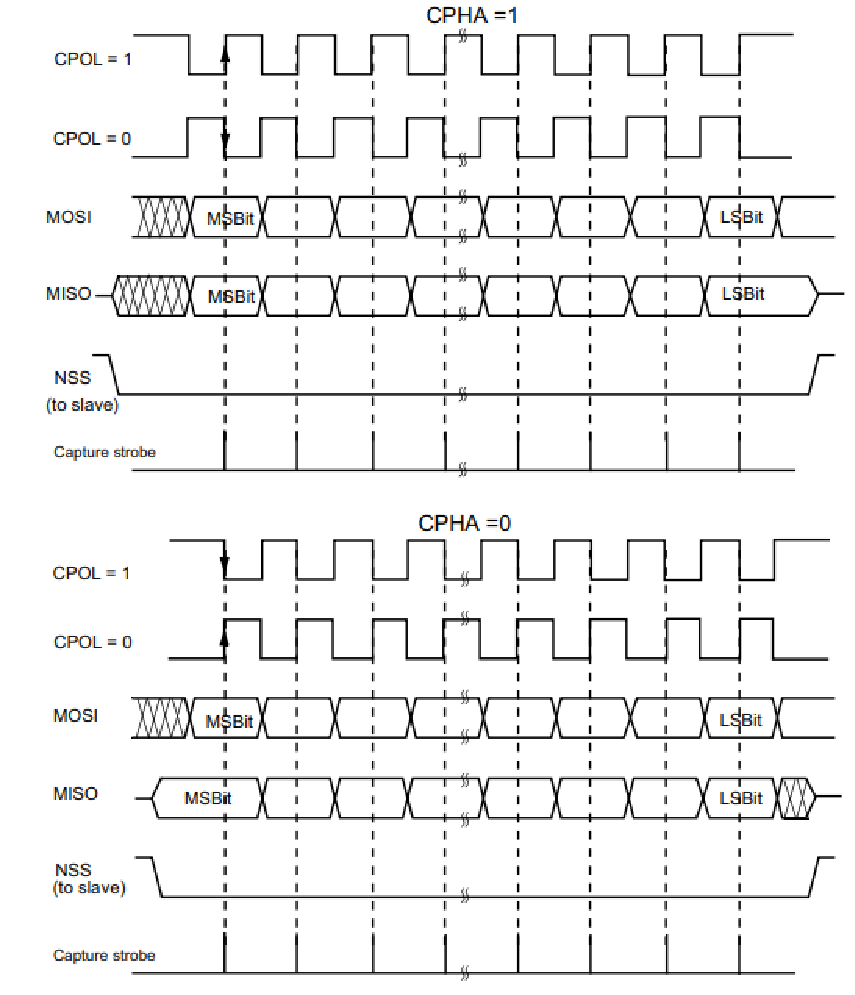
\includegraphics[width=\linewidth]{subfiles/imgs/IP_Blocks_Pics/spi_signal_diagram.pdf}
    \caption{Table of signal timings in the SPI protocol for different values of CPHA and CPOL (Courtesy of STMicroelectronics \cite{SPIManualSTM}).}
    \label{fig:spi_timings}
\end{figure}

Due to the simple protocol, the essential hardware is equally simple. The main component is a shift register which will perform the transmission. Besides this two buffer registers is needed for holding the message and saving the message coming from the slave. A baud rate generator is also needed to create the SCLK signal, which is essentially a counter. Only a single shift register is in theory needed, as the slave also contains a shift register and these two can be connected in a ring connection using MOSI and MISO. An example of this ring connection can be seen in \ref{fig:spi_min_comp}.

\begin{figure}[H]
    \centering
    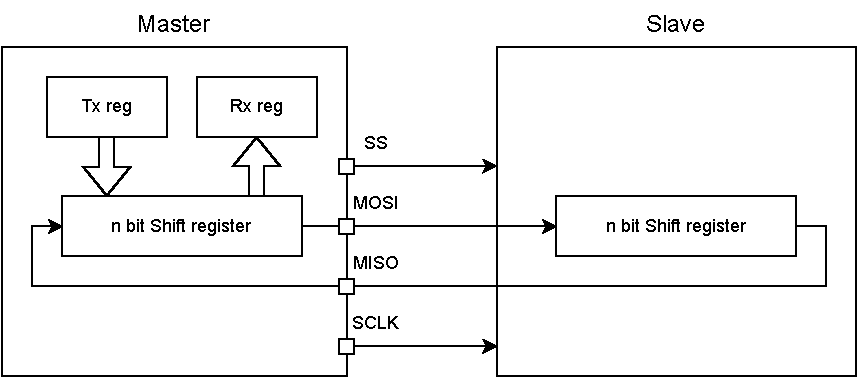
\includegraphics[width=\linewidth]{subfiles/imgs/IP_Blocks_Pics/spi_min_comp.drawio.pdf}
    \caption{Shows the ring connection established by connecting MOSI and MISO to shift registers.}
    \label{fig:spi_min_comp}
\end{figure}

A few modifications and additions will be made to this setup to make it easier to use and to simplify the development. First is the addition of two FIFOs instead of a single transmission register and receiver register. This means that many messages can be written over a short time frame without the need to let the transmitter finish sending the previous message. The rx FIFO removes the necessity of reading the master peripheral each time a new message is received and limits the risk of losing data if new messages are received. Furthermore, even though it is possible to do it with one shift register in the master controller, it is chosen to do it using two shift registers, one for tx and one for rx. This is done to simplify the controller needed for executing the protocol. The extra cost in form of a shift register is deemed insignificant. For selecting the slave it is chosen to use a register for controlling which wire is pulled low. The resulting master block diagram can be seen in figure \ref{fig:spi_func_dia}. 

\begin{figure}[H]
    \centering
    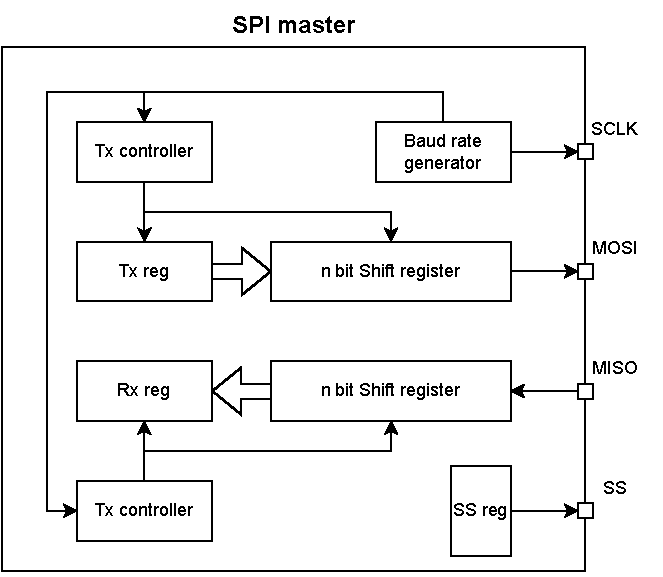
\includegraphics[width=0.75\linewidth]{subfiles/imgs/IP_Blocks_Pics/spi_block_dia.drawio.pdf}
    \caption{Shows functional block diagram of the SPI master that is to be developed. The hollow arrows symbolize a bus connection which is 32 bits wide.}
    \label{fig:spi_func_dia}
\end{figure}


With the functional units established for the system, it is time to discuss the programmable control registers and status registers for the system. The system should be adjustable to a high degree of freedom to ensure that it has a high amount of use cases. First, it should be possible to adjust the clock frequency of the system by controlling the baud rate generator. This will be done in the power of 2's, so that the clock is divided by 2, 4, 8, and so on. Up to and with $2^{16}$. A minimum division of 2 is needed, since the tasks in the form of sampling and shifting, are performed in every period of the SCLK. This means that at least two rising edges from the system clock are needed since everything should update on the system clock and on rising edges. This allows a high range of possible frequencies for the system to run at. It is also worth mentioning here, that the baud rate generator will not generate a clock signal for the system, but will function as an enable signal for the rest of the system which still runs on the system clock. This avoids creating multiple clock domains. 

It should also be possible to adjust the size of the data frames used in the communication, i.e. how many bits are sent between master and slave. This is chosen to be 8, 16, 24 or 32 bits. To this an enable signal is also added, such that the block will not start a transmission before it is intended. Two more control signals are added, which are commonly found in an SPI master, which is clock phase (CPHA) and clock polarity (CPOL) \cite{SPIManualSTM}. These two signals both affect how the SCLK signal is generated and how the shifting and sampling is done. The effects can be seen in figure \ref{fig:spi_timings}. These control signals make the SPI communication highly flexible and it is, therefore, able to communicate with a wide range of different systems.

All control signals from before are bundled into 1 programmable control register. In addition to this, a status register is added, containing the full and empty signals from the two FIFOs and a busy signal to indicate whether a transfer is in progress. To complete the list of registers available to the APB interface, a read and write register is added, which writes to the tx FIFO and reads from the rx FIFO. This list of registers is described extensively in RDL file for the SPI master in GitHub repository.

The programmable control registers and the functional units have been presented and development of the system can begin.

\subsection{Development}
The functional units will be developed in Verilog with a focus on behavioral development, i.e. no direct instantiation of adders, registers, etc. The development has been split into 5 groups: the APB interface, the FIFOs, the rx controller, the tx controller, and the baud rate generator. The FIFOs will be reused from the UART (see section \ref{uart_sec}). 

\subsubsection{TX \& RX Controller}
The tx and rx controllers for the shift registers are simple in design as the ticks needed for performing their respective action are generated by the baud rate generator. Therefore it only needs two states: idle and tx. In idle it simply keeps checking the value of tx\_start and if it's true, it will load in the data available in the FIFO and set a variable t to 0 and set high a tx\_data\_read. The tx\_start is the output of and gate, where the two input signals enable and tx\_fifo\_not\_empty. The tx\_data\_read is set high for one clock cycle to indicate to the FIFO that the value has been read. The next state is the tx. In this state, it performs actions every time a tx\_tick is received. Every time a tick is received, it checks how many times it has performed a shift operation. If it has done it x amount of times it sets a tx\_done signal high and checks whether tx\_start is high. If it is high it sets t to 0 and loads in new data and generates a high tx\_data\_read signal. This is done to enable continuous transmissions instead of resetting to the idle state between each transmission. However, if tx\_start is not high, it goes back to the idle state. If t was not equal to x in the first place, it adds 1 to the value of t and performs a left shift operation on the data. The value of x is decided by the DFS register, which selects the size of the data frame for transmission. All of this information is encapsulated in the ASM chart for the tx controller seen in figure \ref{fig:spi_txctrl}.  
\begin{figure}[H]
    \centering
    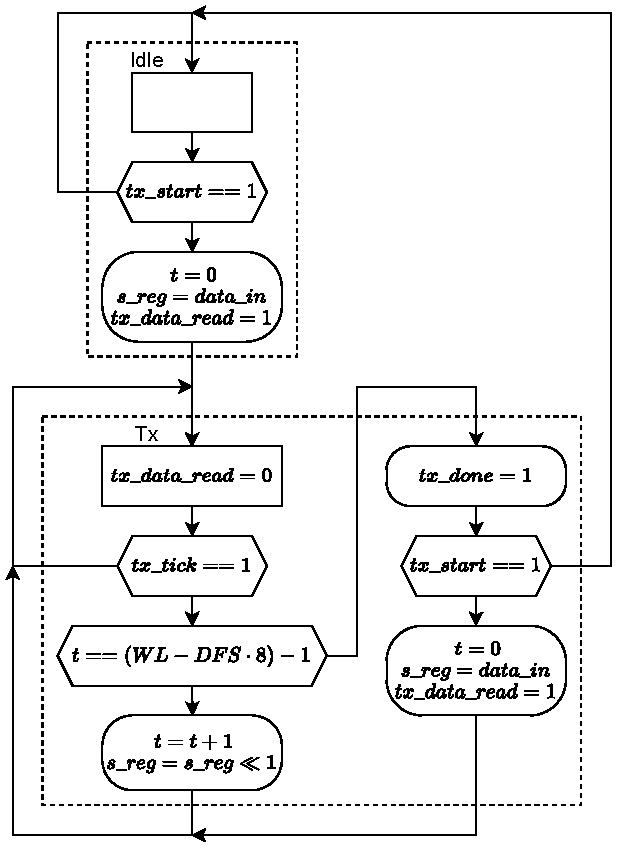
\includegraphics[width=0.5\linewidth]{subfiles/imgs/IP_Blocks_Pics/spi_txctrl.drawio.pdf}
    \caption{Shows the ASM chart for tx controller for the SPI master.}
    \label{fig:spi_txctrl}
\end{figure}

A nearly identical ASM chart can be made for the rx controller. Instead of shifting out data on the tx\_tick, it samples data on the rx\_tick into a shift register. When it has sampled that x amount of times, it saves it into the rx FIFO. 

\subsubsection{Baud Rate Generator}
The task of the baud rate generator is to create the clock signal: SCLK. To do this it has to take the state of the enable signal, the state of the FIFOs, the desired clock frequency, and the CPOL and CPHA signals. Here, it is worth highlighting how the desired clock frequency and CPHA are incorporated into the system. The clock division can be achieved by a simple 16-bit counter from which the output can be taken from a single-bit position depending on the desired division. Therefore the SCLK can simply be generated by connecting all bit positions from the counter to a multiplexer, where the select bits are connected to the BR\_DIV register. However, the output does need to be inverted, as the clock signal has to start with a change, i.e. rising edge in the case of no polarity changes. This is not achieved by the counter itself as it needs to count halfway before a change is made. To fix this, the output from the counter is inverted. 

To achieve correct timing of sampling and shifting, the counter will be reset at the value $2^{BR\_DIV+1}-1$, and either a tx tick or an rx tick will be produced. Which one depends on the value of CPHA. One is added to the exponent since the smallest divider is 2. At the halfway point of the count, the other tick will be produced. To incorporate CPHA fully, it will decide one of two states enter when coming from idle. These two states will differ on whether the clock is activated instantly or delayed by half a clock cycle. Thereby, the desired phase change is achieved.  

With the details discussed and elaborated, an ASM chart is made as seen in figure \ref{fig:spi_brg}, which encapsulates the operation of the baud rate generator. The Verilog code is written based on this ASM chart.    

\begin{figure}[H]
    \centering
    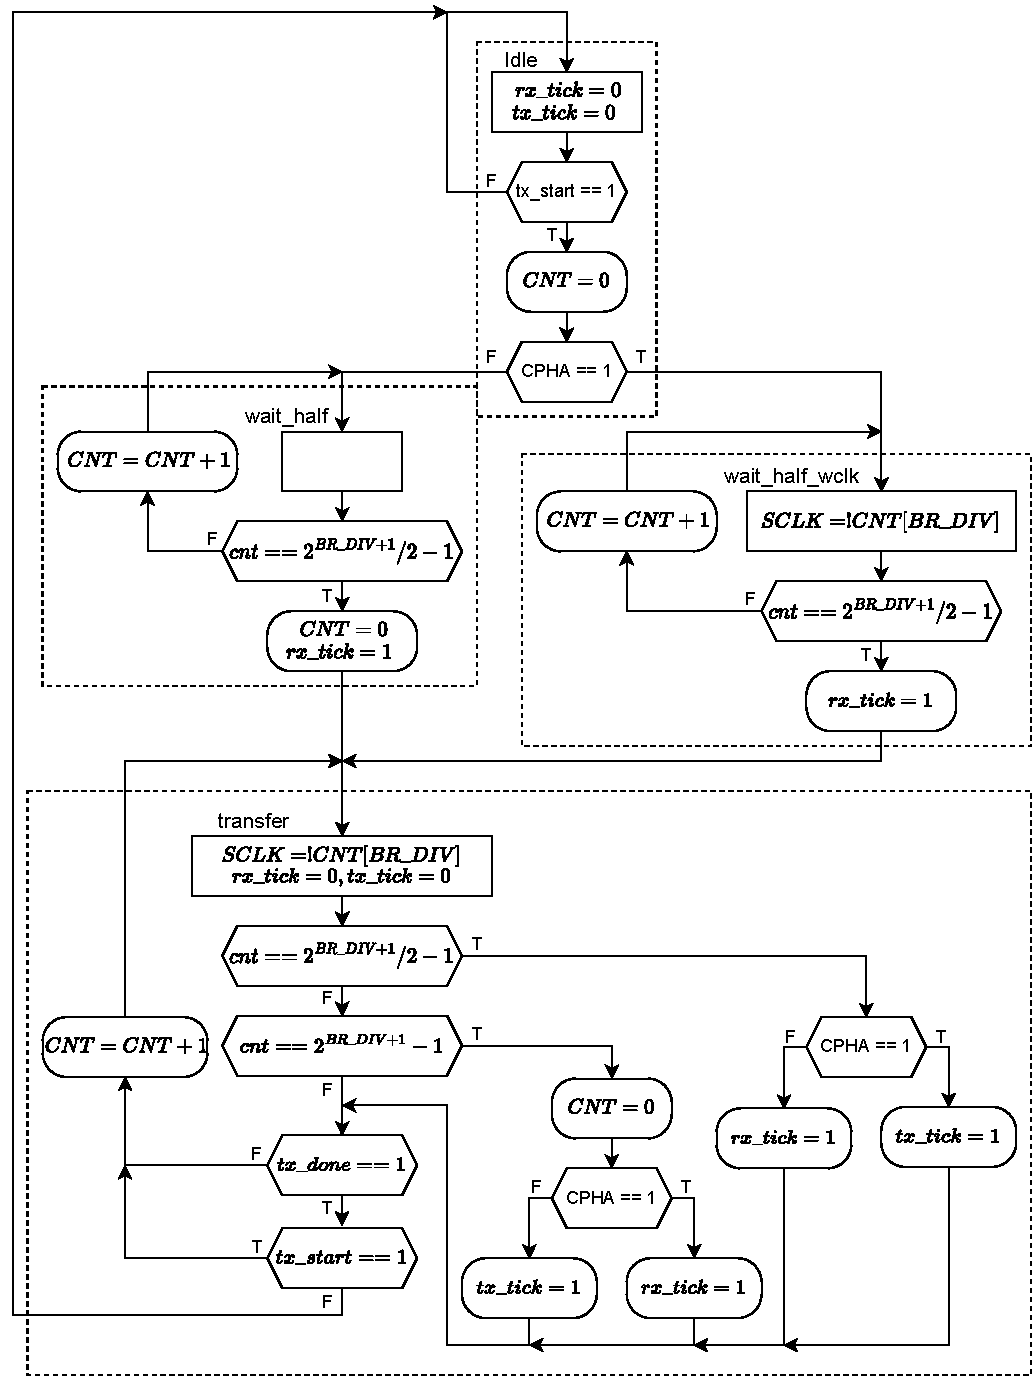
\includegraphics[width=\linewidth]{subfiles/imgs/IP_Blocks_Pics/spi_brg.pdf}
    \caption{Shows the ASM chart for the baud rate generator in the SPI master.}
    \label{fig:spi_brg}
\end{figure}

%\subsection{APB Interface}
%In the APB interface, the functional units are connected to create the full system. These units are the rx controller, tx controller, the baud rate generators and two FIFOs, one for rx and one for tx. The registers describes in table \todo{add register table} are then added and connected to APB interface. The APB interface is set up as previously described in section \ref{apb_if}. The PREADY is permanently set as to avoid stalling of the CPU. A PLSVERR signal is generated if one tries to write to the FIFO while it is full or read from it when it is empty. 

\subsection{UVM Verification}
The verification of the SPI master follows the same procedure as the verification of the UART controller. Doing development it has been under constant simple verification using the PicoRV32 and C++, to ensure that basic functionality is achieved. Following this basic verification, a more extensive verification is set up using the UVM environment. For the UVM environment, an agent consisting of a driver, sequencer and monitor, a scoreboard with reference module, and test sequences has been developed. 

The UVM driver is designed to produce the signals expected from a connected slave, so it only generates the MISO signal. It does this by shifting out individual bits starting with MSB. The shifting occurs at a rising edge of the system clock. Which specific rising edge is calculated based on the data frame size, baud rate, CPOL, and CPHA. It was a priority to make the shifting independent of the SCLK signal, as using this signal to do the shifting would mean that an error on SCLK is more likely to go undiscovered. The monitor samples the MOSI signal, again, based on the system clock, data frame size, baud rate, CPHA, and CPOL being independent of the SCLK signal again. The sequencer used is the basic version supplied with the UVM environment.

The scoreboard samples the signals sent using the APB interface or the SPI interface. These signals are then compared to the reference module and if they are different an error is reported. The scoreboard has two coverage groups, an APB coverage group, and an SPI coverage group. The APB group covers the read and write operations performed through the APB interface. The SPI group covers the status of CPOL, CPHA, the data frame size, and the baud rate used. A cross-coverage group is made using these four signals, such that it can verify at what CPOL, CPHA, and data frame size a specific baud rate has been tested. The reference module consists of the internal registers of the SPI master based on the RDL file for the SPI master. Whenever a change to the registers is made, this is reported to the driver and monitor such that they can change settings as well to match what the DUT is doing. 

The test sequences of the SPI master consist of writing data through the APB interface and the SPI slave interface. Random data is sent to the driver at all times using a UVM item. Every time an item is sent, the test sequence waits for this item to complete before a new item is created. This ensures that the slave will always respond with a known item when a transfer is initiated from the DUT. The main test sequence is through the APB interface. It will start the test by setting a baud rate. Then it will write multiple random messages to the MOSI FIFO and start transmission. Multiple messages are written to test the SPI master's capabilities for continuous transmission. When this is done it changes CPOL repeats. This is again repeated for CPHA and the 4 possible data frame sizes. When it has tested a specific baud rate, it moves on to the next baud rate and repeats. 

The resulting coverage report generated by using the UVM environment for verification of the SPI master can be seen in appendix \ref{spi_cov_rep}. After verification of the basic HDL code, the triplicated version of the SPI master was designed and tested again. An identical coverage report was generated. 





%%%%%%%%%%%%%%%%%%%%%%% UART %%%%%%%%%%%%%%%%%%%%%%%%%%%%%%%


\section{UART Controller}
\label{uart_sec}
In this section, a UART (Universal Asynchronous Receiver/Transmitter) controller will be developed. The UART controller will be connected to the CPU as a peripheral interface on the APB bus. The development of the UART controller is inspired by "FPGA Prototyping by Verilog Examples" \cite{FPGAprototyping}. 

A UART controller is asynchronous due to the fact that no clock signal is transmitted. Therefore it only makes use of 1 input and 1 output wire, rx and tx respectively. To achieve a successful transmission the protocol makes use of a common symbol frequency, commonly referred to as baud rate, and start, data and stop bits of predefined length. A parity bit can also be included for error detection. The common ranges for these values can be seen in figure \ref{fig:uart_signals}. In this protocol the idle is logic level high, meaning that the start bit is created by pulling the signal line low, indicating that a transmission is starting. The LSB is transmitted first in the UART protocol. For this controller, it is decided to use a data frame size of 8 bits, no parity bit, and 1 stop bit. The parity bit is not utilized, as the rx and tx lines will be fully triplicated. To allow flexibility in the communication, the baud rate should be changeable on the fly, i.e. while the system is running.     

\begin{figure}[H]
    \centering
    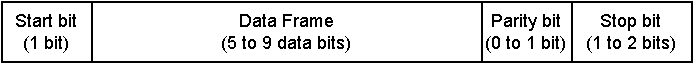
\includegraphics[width = \linewidth]{subfiles/imgs/IP_Blocks_Pics/uart_signals.drawio.pdf}
    \caption{Shows the common ranges for the length of different sections of the UART protocol \cite{AnalogUART}.}
    \label{fig:uart_signals}
\end{figure}

The UART controller itself consists of 5 elements: A baud rate generator, a transmitter module, a receiver module, and two first-in, first-out (FIFO) buffers. The interconnection between these elements can be seen in figure \ref{fig:uart_bd}.

\begin{figure}[H]
    \centering
    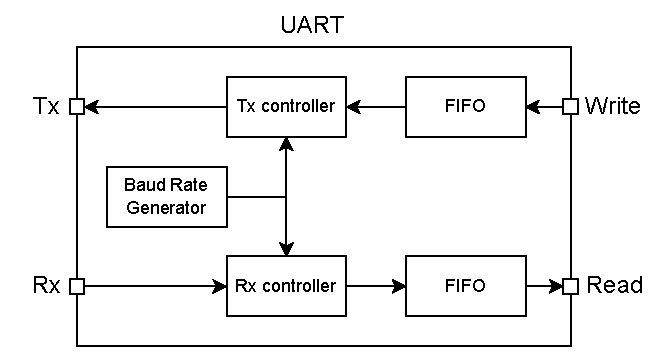
\includegraphics[width=0.7\linewidth]{subfiles/imgs/IP_Blocks_Pics/uart_bd.drawio.pdf}
    \caption{Block diagram of the UART components and their connections.}
    \label{fig:uart_bd}
\end{figure}

To control the system, programmable control register will be used and made accessible from the APB interface. The specific control registers have been chosen based on the components used in the controller and the common use case. As this is a fairly simple system in itself, only 3 programmable registers and a status register are implemented. These consist of writing and reading from the FIFO buffers in the system, setting the baud rate, and reading the status of the aforementioned FIFO buffers. This implementation of the control registers and their exact layout are summarised in the table \ref{tab:uart_regs}.

\begin{table}[H]
\centering
\caption{Shows the programmable register layout available to the APB interface for the UART controller. Addresses are given in hexadecimal.}
\label{tab:uart_regs}
\begin{tabular}{l|l|l}
\textbf{Field name}      & \textbf{Address} & \textbf{Description} \\ \hline
status          & 0x00    & \makecell[l]{Read only: Holds the status values for the rx and tx \\ FIFOs and an additional busy signal}            \\ \hline
read\_rx\_data  & 0x04    & \makecell[l]{Read only: reads the values currently in the \\ rx FIFO. Returns an error if the FIFO is empty}            \\ \hline
write\_tx\_data & 0x08    & \makecell[l]{Write Only: Writes data to the tx FIFO, \\ which begins transmission. Returns error if FIFO is full.}            \\ \hline
set\_baudrate   & 0x12    & \makecell[l]{Write and read: Sets the baud rate of the UART \\ or reads the currently used baud rate.}         
\end{tabular}
\end{table}

The higher-level architecture has now been described and the next step is to begin the HDL implementation of each of the functional units.

\subsection{Baud Rate Generator}
The baud rate generator is used to generate the ticks for the rx/tx controller. This will be done by taking the system clock and dividing it by a specific amount to reach the specified baud rate. This division is done using a mod-m counter and the m value can be calculated as seen in equation \ref{divisor_calc_uart}.

\begin{equation}
    \label{divisor_calc_uart}
    m = \frac{clk}{os \cdot baudrate}
\end{equation}

Where:
\begin{table}[H]
\begin{tabular}{ll}
$m$ is the value which the counter should reset at & \\
$clk$ is the frequency of the system clock & $[Hz]$\\
$os$ is the oversampling rate & \\
$baudrate$ is the specified baud rate & $[\frac{bit}{s}]$
\end{tabular}
\end{table}

As the baud rate is programmable, a list of 8 possible baud rates has been chosen, which the baud rate generator is capable of generating. These baud rates are chosen on the premise of commonly used baud rates with a bias towards higher baud rates. They are as follows: 4800, 9600, 19200, 38400, 57600, 115200, 128000, and 256000. The choice is arbitrary and can always be changed by modifying a simple list in the Verilog source file. These baud rates, together with the clock frequency and oversampling rate, can be used to calculate the values for when to reset the counter (m). These are calculated at compile time using equation \ref{divisor_calc_uart} and saved in an array. From these m values, the needed bit width for the counter and all other relevant signals in the baud rate generator. The baud rate can then be changed by programming the corresponding register to a different binary value. The m value will then be updated and the counter will be reset. Resetting the counter eliminates the risk of changing m to a lower value than the current count. This would result in the counter overflowing before normal operation would resume. This does not eliminate the risk of the baud rate being changed in the middle of a transmission. To eliminate this, the baud rate will not be changed while a busy signal is high. This busy signal will come from the rx and tx controllers and will indicate whether they are idle or not.

From this description, a functional diagram has been derived which can be seen in figure \ref{fig:uart_func_dia}. This will be used as a baseline for the behavioral modeling in Verilog.

\begin{figure}[H]
    \centering
    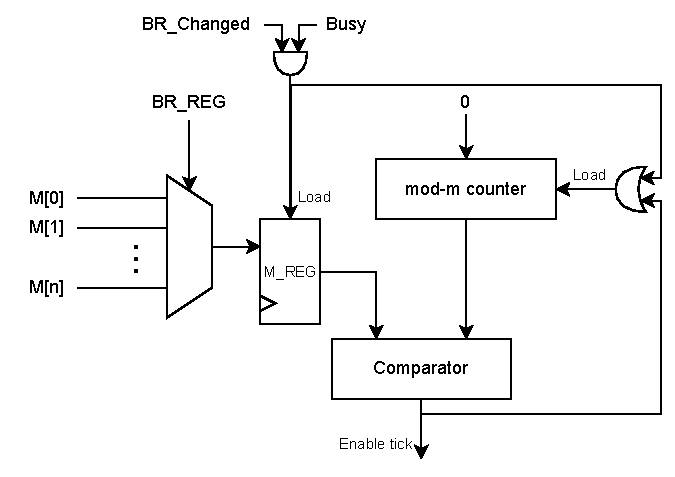
\includegraphics[width=0.9\linewidth]{subfiles/imgs/IP_Blocks_Pics/uart_func_dia.drawio.pdf}
    \caption{Shows a functional diagram for the baud rate generator. This is used to highlight the purposed functionality in an easy-to-understand way and therefore might not be the optimal solution.}
    \label{fig:uart_func_dia}
\end{figure}

\subsection{First In First Out buffer}
The first in first out (FIFO) buffer will for storing the received words and the words to transmit. This allows for a far more flexible usage of the UART, by not required to read the received words immediately and by allowing multiple words to be written to the UART from the CPU. The implementation will be based on a circular queue. This implementation illustrates the operation by taking a range of memory elements and forming them into a single. Two pointers will then be created, one for read operation and one for write operation. When one of these operations is performed the corresponding pointer will increase by one. This continues until the last memory element is reached, when an operation is then performed the pointer will reset back to 0 and start over again as in a circle. From the positions of the pointers, it is possible to derive the status of the FIFO, whether it is full or empty. It is also possible to rule out the illegal operation using the derived status, as the FIFO cannot be read from when empty and cannot be written to when full. 

The FIFO will be parameterized using two variables. These will be word length, simply how large each memory element is, and the number of address bits, which will control how many memory elements are in the FIFO buffer. The number of address bits will be raised to the power of 2 to create a length that corresponds to a whole number of bits. This ensures that the pointers will overflow by themselves without the need for a checker. 

The FIFO can be described as a state machine with the states being given by the read and write pointers. The next state logic will be given by the control signals: read and write. These control what operations will be performed. 

\subsection{Tx/Rx Controller}
The receiving and transmitting controllers are similar in operation and will therefore be presented together. These controllers will be parameterized using the chosen configuration of the UART protocol. Since parity will not be implemented, the parameters are the number of data bits, the number of stop bits, and oversampling rate.

4 states can be identified for both controllers. These correspond to the sections of the protocol shown in figure \ref{fig:uart_signals} in addition to an idle state. The states are then called: idle, start, data and stop. The idle contains a simple wait routine. For the transmitter this wait routine is broken when the tx FIFO buffer is not empty, communicated to the controller using a signal called tx\_start. The next state is "start", where the transmitter will send a start bit in the form of a binary 0. This will last for an amount of enable ticks received from the baud rate generator corresponding to the oversampling rate, i.e. if the oversampling rate is 16, the controller will count 16 enable ticks from the baud rate generator before moving to the next state. In the next state, the data is sent, with LSB being sent first. Each data bit has the same duration as the transmitted start bit. This is done the number of times specified by the number of data bits given as a parameter. The last state is the stop state, where a 1 is transmitted for the duration specified by the number of stop bits. Each bit has the length specified by the oversampling rate. This operation is encapsulated in the ASM chart shown in figure \ref{fig:uart_tx_asm}.

\begin{figure}[H]
    \centering
    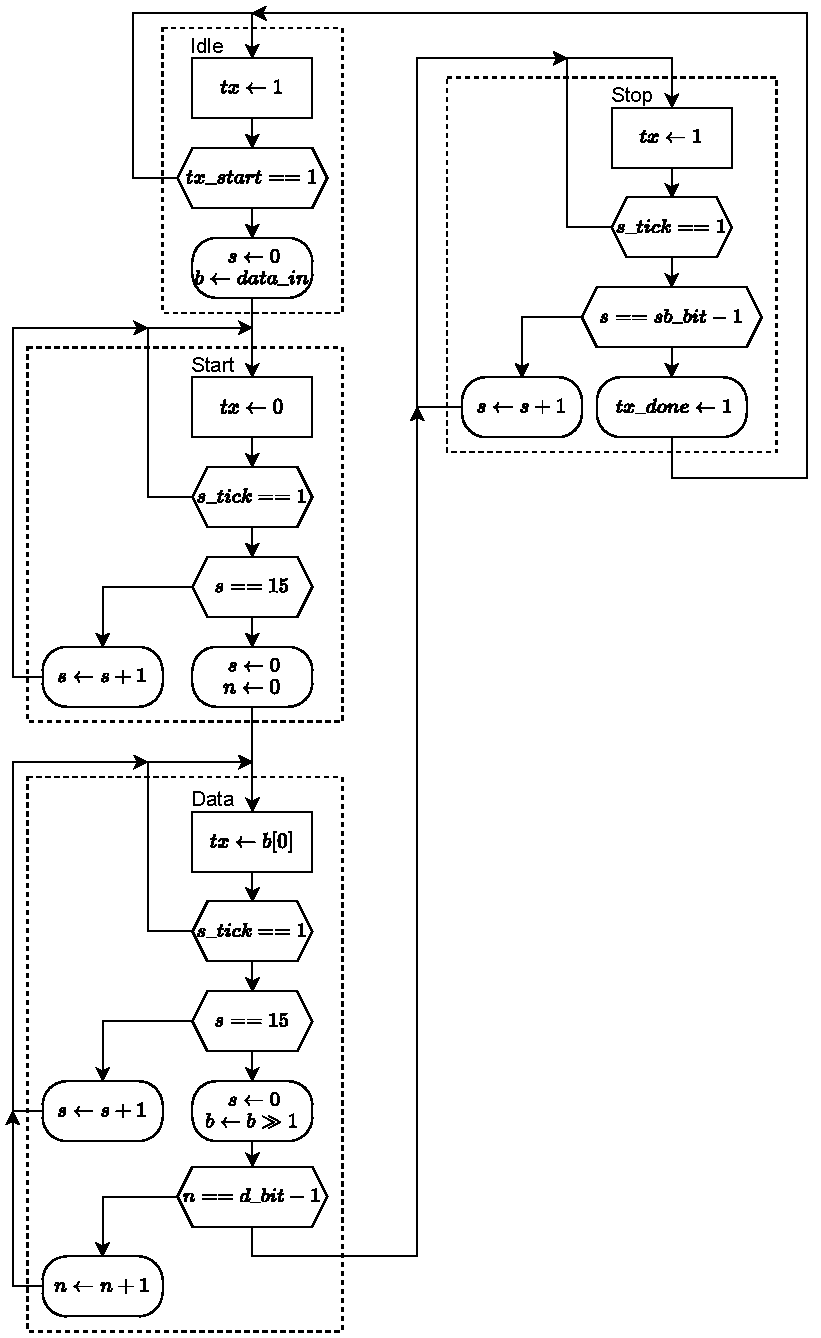
\includegraphics[scale=.9]{subfiles/imgs/IP_Blocks_Pics/UART_tx.drawio.pdf}
    \caption{ASM chart for a UART transmitter without parity bit.}
    \label{fig:uart_tx_asm}
\end{figure}

For the receiver, the ASM is nearly identical and will therefore not be shown. However, the differences will be highlighted here. For the rx controller, the idle state will be broken when the rx line goes low, corresponding to receiving the start bit. The start state will only count half of the enabled ticks specified by the oversampling rate. This is done such that the sampling of the rx line will be done in the middle of the data bit duration, ensuring that hold and setup times will not be violated. 

\subsection{Verification of UART Controller Design}
The verification will be done in multiple steps. Critical functionality needed for basic operation will be tested using a Verilog testbench already developed which uses the PicoRV32 (CPU core). When basic functionality is ensured, a more elaborate testing environment will be designed using UVM.

By using the PicoRV32 for verification of basic functionality, the task is made easier by allowing for the use of the APB bridge attached to the PicoRV32 and allowing for the use of the c++ programming language. This makes writing the APB interface of the UART controller a one-line operation, while if one had used a Verilog testbench, this would require many lines of code. This does however rely on the correct operation of the CPU and the APB interface, but as these have both been verified before, this is not an obstacle. To provide stimuli to the output and monitor the output of the UART controller, a copy of the UART has been connected to the tx and rx lines. This copy of the UART does not make use of the APB interface as this is just an object used for testing purposes. This simplifies the production of the stimuli and monitoring of the outputs, as it can observe whether data is received correctly and what stimuli are applied, which is used for comparison. One has to be aware of the fact, that this test setup uses the UART itself to test whether the protocol is executed correctly, so errors can go undetected if they do not cause fatal errors in the operation. However, within the scope of basic functionality testing, this is deemed acceptable as this will be tested by the UVM environment. The c++ testbench is seen in code \ref{uart_c_test_code}, while the relevant part of the Verilog testbench containing the test UART is seen in code \ref{uart_verilog_test_code}. 

\begin{lstlisting}[caption={C++ code for basic functionality testing of the UART controller},label={uart_c_test_code},language=C++]
#include <cstdint>

//Base address for the UART on the APB bridge
#define UART_BASE_ADDR 0x0A0C0000

int main(){
    volatile uint32_t *uart_addr = (uint32_t *)UART_BASE_ADDR;
    uint32_t status_reg;
    uint32_t read_reg;
    *(uart_addr+3) = 0x05;
    *(uart_addr+2) = 0xDA;
    status_reg = *(uart_addr);
    *(uart_addr+2) = status_reg;
    while (status_reg == (int)2){
        status_reg = *(uart_addr);
    };
    *(uart_addr+2) = status_reg;
    read_reg = *(uart_addr+1);
    *(uart_addr+2) = read_reg;
    return 0;
}
\end{lstlisting}

\begin{lstlisting}[caption={Verilog code for basic functionality testing of the UART controller},label={uart_verilog_test_code},language=verilog]
//uart test setup
reg rd_uart, wr_uart;
reg [7:0] tx_data;
reg [2:0] BR_REG;
wire rx_empty, rx_full, tx_full;
wire [7:0] rx_data;
uart_top test_uart (
	.clk(clk), .reset(!resetn),
	.rd_uart(rd_uart), .wr_uart(wr_uart),
	.tx_data(tx_data), .rx(uart_tx), 
	.rx_empty(rx_empty), .rx_full(rx_full), 
	.tx_full(tx_full), .rx_data(rx_data),
	.tx(uart_rx), .BR_REG(BR_REG)
);
	
initial begin
	rd_uart < = 1'b0;
	wr_uart < = 1'b0;
	BR_REG < = 3'b101;
	repeat(1000) @(posedge clk);
	tx_data < = 8'h4B;
	@(posedge clk);
	wr_uart < = 1'b1;
	@(posedge clk);
	wr_uart < = 1'b0;
end
\end{lstlisting}

With basic functionality verified, elaborate testing based on UVM will begin development. This development consists of designing the relevant agents with the corresponding monitor, sequencer, and driver, a UART package for sending information between components, a model of the interface, a reference module, and a scoreboard with functional coverage. The UART will need two agents to connect to the test environment, an APB agent and a UART agent. The APB agent will monitor and provide stimuli for the APB interface, while the UART agent will monitor the tx line and provide stimuli on the rx line. Since an APB agent has been developed before, this can simply be reused without any modifications. It only needs to be instantiated and connected to the APB interface of the UART. This highlights some of the advantages of using UVM as this facilitates the reuse of components with its hierarchical structure. 

It is worth mentioning here, that it is a goal to create a test environment that is distanced from the implementation in Verilog, i.e. by using a high-level description of certain parameters used in the functionality of the UART. If the test environment is designed using a low-level language approach similar to the use of Verilog, one has a higher risk of designing the same bugs and mistakes as in the Verilog code, especially when both design and verification are done by the same individual. Each of the mentioned components will now be designed individually, starting with infrastructure-related items and then from the bottom of the hierarchical structure.

\subsubsection{UART Interface}
The interface is extremely simple and only consists of the input wire rx and the output wire tx from the UART. There is no need to define an APB interface as this has already been done before in the development of the APB agent.

\subsubsection{UART Item}
The UART item is a class object, which will be used for packaging the relevant data for a UART transaction and sending it between UVM components. This item will have 3 variables: the data which has been sent, the type of transaction (received or transmitted), and whether the package is valid. 

\subsubsection{UART Sequencer}
The UART sequencer is a part of the agent required for making it active, i.e. capable of driving stimuli to the device under test (DUT). In this test setup, the basic UVM sequencer will be used and therefore no development will be required. The sequencer becomes relevant when multiple sequences are sending packages to the same agent. In this case, it is the task of the sequencer to decide which packages have priority and will be sent to the driver first and in general what the order of packages will be. However, in this simple test environment for the UART, it is not a plan to have multiple parallel running sequences and therefore no special scheduling scheme is necessary. 

\subsubsection{UART Driver}
The task of the driver is to request an item from the sequencer, which will be a class object of the UART item and convert the parallel data into serial data by transmitting it using the UART protocol. This requires that it uses variables for the data length, stop length, parity bit, and the baud rate. All of these are required to be configured to match the configurations of the test UART. Even though parity is not implemented in the designed UART, it is included here, such that the UART has greater reusability in other UVM test environments. The oversampling rate is not a necessary variable here as the driver will not base the baud duration on a clock frequency. Instead, a high-level approach will be used, by simply calculating the baud duration as $1/baudrate$. This ensures a difference in the implementations but does result in the UVM environment not being cycle accurate to the DUT. This is due to the fact, that when the baud rate is used to calculate the count at which to reset the baud rate generator, it is rounded down or up as it can't count to fractional values. It does not result in critical differences in the baud duration, but it does mean the DUT and the test environment might differ for a few clock cycles after transmitting a message. 

\subsubsection{UART Monitor}
The monitor operates nearly identically to the driver. Instead of driving signals to rx line of the DUT, it will sample the tx line. Identically to the Verilog implementation, the monitor will wait a half baud duration, when a start bit is encountered. Following that, it will wait for the full baud duration between sampling. This is done to sample in the middle of a baud. Due to the exact same reason as in the driver, the monitor will have slight differences in when a message is received and might not be accurate compared to the DUT in a few clock cycles following a transmission.  

\subsubsection{UART Agent}
The UART agent is the container of the sequencer, driver, and monitor. One thing worth mentioning is that the agent will also have the variables for baud rate, data length, stop length, and parity. The agent will then pass these down to the components within the agent. This is done such the components of the agent can be configured by only configuring the agent.

\subsubsection{Scoreboard and Reference Module}
The scoreboard contains the reference module, the functional coverage, and the checking mechanisms to compare the reference module and the DUT. The scoreboard will contain subscribers for the APB and the UART interface. That is to say, it will receive the packages sent using both interfaces. These packages will then be used to update the reference module or check if the reference module and DUT are identical. Each time a package is received, it will sample the functional coverage, which will add one to the correct bin corresponding to the action performed. First, the functional coverage will be discussed and then the reference module and checking mechanisms.

The functional coverage, as the name implies, is a metric used to show how well the DUT has been tested on its different functionalities. This can be combined with code coverage to form a metric for how extensively the DUT has been tested. The functional coverage will be subdivided into two categories: APB and UART, corresponding to the two interfaces on the DUT. The UART coverage group will only be characterized by received messages and transmitted messages. The APB coverage will be divided into 3 categories: read, write and errors. The read-and-write category will contain all the programmable control registers of the DUT. The status registers have been divided further into all the possible combinations of status signals (Excluding the busy signal). As some of them are illegal, they have been marked this way, meaning that the success criteria become avoiding that state. The reading of the received messages (RX FIFO) together with the writing of messages to transmit (tx FIFO) has been divided into all the possible messages to send using 8 bits. This makes it possible to track what message has been sent. The error category is used to test whether correct errors are received when trying to write to a full tx FIFO or reading from an empty RX FIFO. 

Next, is the design of the reference module. This reference module is used for comparison when testing the DUT. As the transmitting and receiving of the message are handled by the UART agent, the only things needed to be modelled by the reference module are the registers inside the DUT. The FIFO can be modelled by a std::queue in C++. Every time a message is received from the UART or APB agent or an APB interface operation is performed, the contents of these queues will be updated together with the status signals empty and full. The length of these queues will be equal to that of the FIFOs in the DUT. The busy status is excluded here as modelling this signal, would require a higher level of communication between the agent and the scoreboard. The development time of this system is not deemed necessary as the busy signal is not a critical feature. The rest of the registers can be modelled as simple variables.

The checking mechanisms are performed every time an APB read operation is performed or a message is received on the UART monitor. Every time a message is received on the UART monitor, the first item of the queue modelling the tx FIFO is popped (read and removed) and compared to the received message and the status variables are updated. When an APB read operation is performed, the comparison depends on which register was read. In the case of reading the rx FIFO, an operation equivalent to that of receiving a message on the UART monitor is performed on the respective queue object. When reading the status or baud rate register (BR\_REG), the corresponding variable is used for comparison. The error signals are also checked doing APB read operations as these are subpart of the APB interface. If an error occurs, meaning that the DUT and reference module are not equivalent, it is reported to the user.

\subsection{Test sequences}
The UVM environment has now been designed and the development of test sequences (Stimuli for the DUT) can begin. The tests will be split into 3 categories: status test, error test and UART test. The status test will ensure that all states of the FIFOs are reached to ensure correct operation. The error test will ensure that the error signals are received from the APB interface at the correct times, i.e. reading from an empty FIFO and writing to a full FIFO. The UART test will write to tx FIFO using the APB interface and transmit a message using the UART driver using random data. The resulting coverage report from using these test sequences can be seen in appendix \ref{uart_cov_rep}. 

\section{Triplication}
Triplication of the UART was done using the TMRG tool. For this tool to function all registers in the Verilog code would need altering. For each register, a wire was added named the same as the register, but with an added "Voted" to the end of it. The voted wire was then used everywhere the original register is used as an input. This allows the TMRG tool to triplicate those registers.

Doing triplication it was discovered that the TMRG tool does not allow for the Verilog function structure. This made the baud rate changing feature fall apart, as a function was used to calculate the count at which the counter should reset. Another approach was needed. Instead, Python was used to generate the mod-counter, the uart\_top, and the apb\_uart file based on a given set of baud rates. This is a lot more flexible than the original approach but does make the changing of the source code harder, as this now needs to be changed inside the python template. The Python file uses two templates: one for a single baud rate and one for multiple baud rates. This python file is integrated into the compilation of the entire project, such that every time the project is compiled, the python file is used to generate the mod-m counter given a range of defined inputs. 

Both the triplicated version with a single baud rate and one with multiple baud rates are tested using the UVM environment. The exact same coverage report is achieved in these tests and can be seen in appendix \ref{uart_cov_rep}.

\section{Physical Implementation}
The last step of development for the UART is the physical implementation. This follows the steps described in section \ref{phys_imp_theory}. The die size is \SI{110}{\um} by \SI{110}{\um} including power rings. The I/O connections have been spaced equally around all four sides of the die. Dynamic power analysis using a testbench has been performed and IR drops have been analyzed. The overview of the results of this process can be seen in figure \ref{fig:uart_phys_impl_stats}. A figure of the IR drop can be seen in \ref{fig:uart_irdrop}. The design violates no hold or setup timings at \SI{325}{MHz}, it has \SI{88.35}{\%} utilization of area, and uses \SI{0.61}{mW}.

\begin{figure}[H]
    \centering
    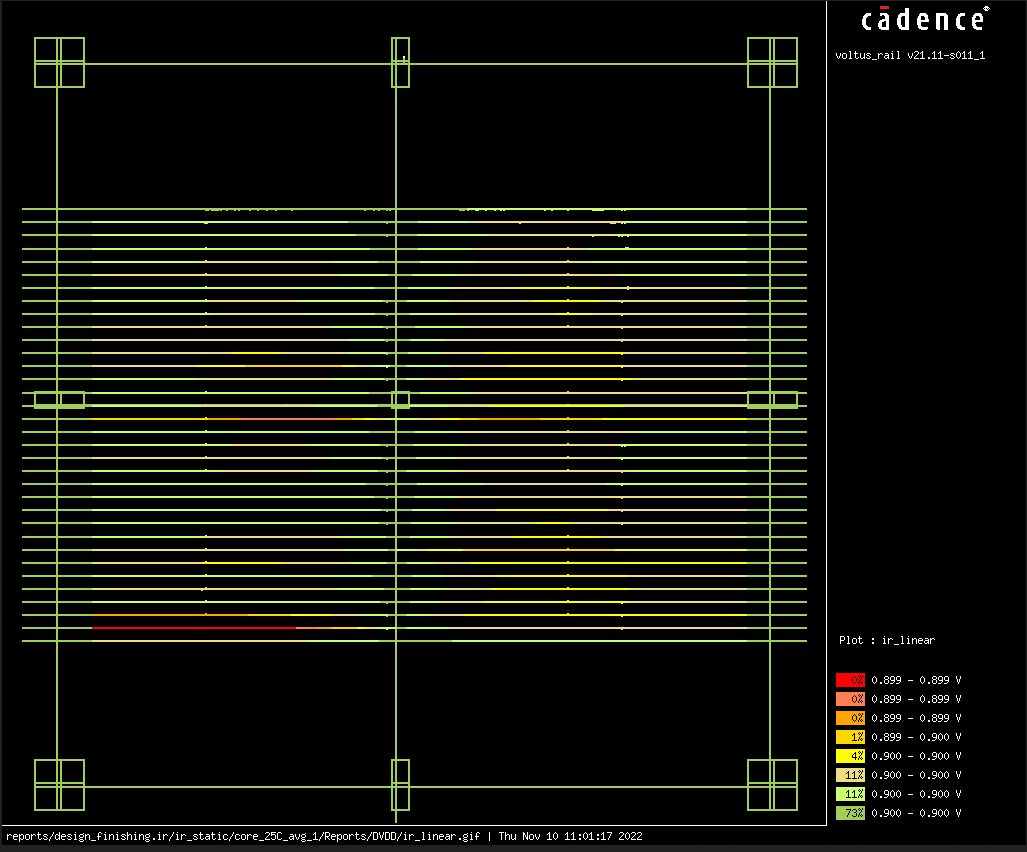
\includegraphics[width=0.85\linewidth]{subfiles/imgs/IP_Blocks_Pics/irdrop.PNG}
    \caption{Shows the IR drop for the physical implementation of the UART controller. Even though some areas are red, the percentage drop is minimal.}
    \label{fig:uart_irdrop}
\end{figure}

\begin{figure}[H]
    \centering
    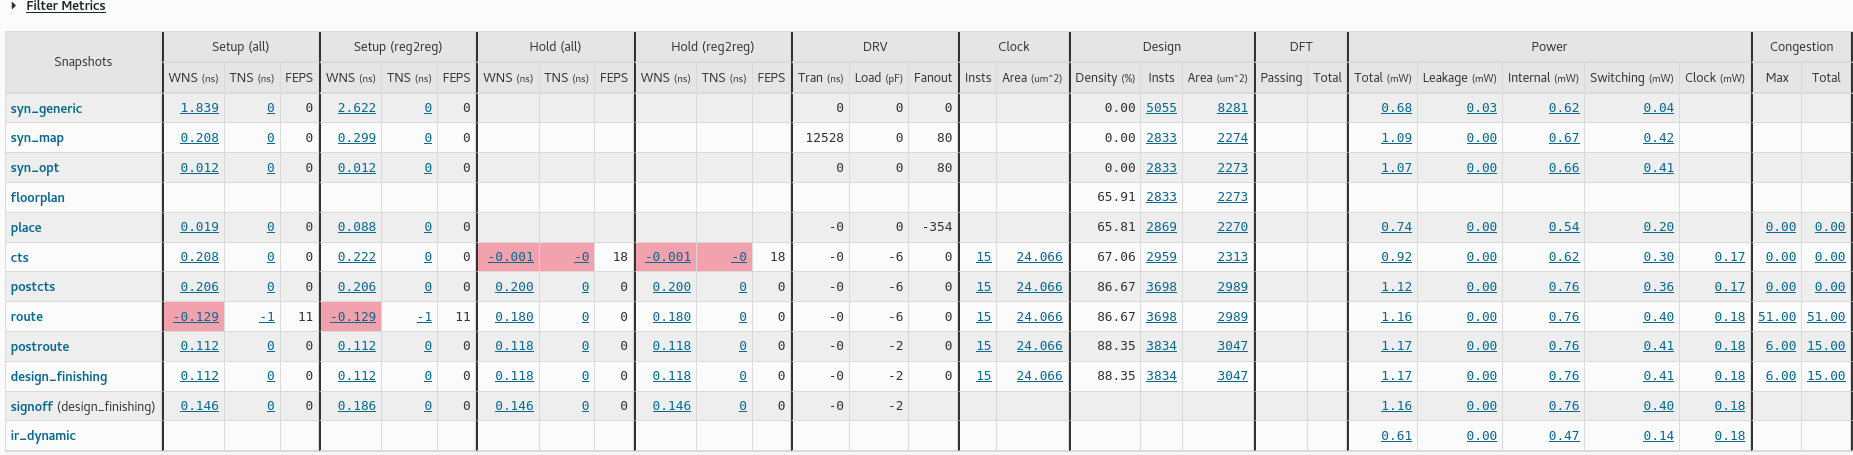
\includegraphics[scale = 0.4, angle =90]{subfiles/imgs/IP_Blocks_Pics/impl_data.PNG}
    \caption{Shows the table of results relevant to the physical implementation.}
    \label{fig:uart_phys_impl_stats}
\end{figure}



%Introduction, blocks will be designed to widely usable
% APB interface
% BLOCK:
% Explain protocol/features
% Components
% Ctrl registers
% Actual design
% Verification
% 

\end{document}
